\subsubsection{Modification de chaînes (Win32)}

Nous pouvons facilement trouver la chaîne ``hello, world'' dans l'exécutable en utilisant Hiew:

\begin{figure}[H]
\centering
\myincludegraphics{patterns/01_helloworld/hola_edit1.png}
\caption{Hiew}
\label{}
\end{figure}

Et nous pouvons essayer de traduire notre message en espagnol:

\begin{figure}[H]
\centering
\myincludegraphics{patterns/01_helloworld/hola_edit2.png}
\caption{Hiew}
\label{}
\end{figure}

Le texte en espagnol est un octet plus court que celui en anglais, nous ajoutons l'octet 0x0A à la fin
 (\TT{\textbackslash{}n}) ainsi qu'un octet à zéro.

Ça fonctionne.

Comment faire si nous voulons insérer un message plus long ?
Il y a quelques octets à zéro après le texte original en anglais.
Il est difficile de dire s’ils peuvent être écrasés: ils peuvent être utilisés quelque part dans du code \ac{CRT},
ou pas.
De toutes façons, écrasez-les seulement si vous savez vraiment ce que vous faîtes.

\subsubsection{Modification de chaînes (Linux x64)}

\myindex{\radare}
Essayons de modifier un exécutable Linux x64 en utilisant \radare{}:

\lstinputlisting[caption=\radare{} session]{patterns/01_helloworld/radare.lst}

Ce que je fais ici: je cherche la chaîne \q{hello} en utilisant la commande  \TT{/},
ensuite je déplace le \emph{curseur} (ou \emph{seek} selon la terminologie de \radare{}) à cette adresse.
Je veux être certain d'être à la bonne adresse: \TT{px} affiche les octets ici.
\TT{oo+} passe \radare{} en mode \emph{read-write}.
\TT{w} écrit une chaîne ASCII à la \emph{seek} (\emph{position}) courante.
Notez le \TT{\textbackslash{}00} à la fin--c'est l'octet à zéro.
\TT{q} quitte.

subsubsection{Ceci est une histoire vraie de modification de logiciel}
\myindex{\SoftwareCracking}

Un logiciel de traitement d'image, lorsqu'il n'était pas enregistré, ajoutait un
tatouage numérique comme ``Cette image a été traitée par la version d'évaluation
de [nom du logiciel]'', à travers l'image.
Nous avons essayé au hasard: nous avons trouvé cette chaîne dans le fichier exécutable
et avons mis des espaces à la place.
Le tatouage a disparu.
Techniquement parlant, il continuait d'apparaître.
\myindex{Qt}
Avec l'aide des fonctions Qt, le tatouage numérique était toujours ajouté à l'image
résultante.
Mais ajouter des espaces n'altérait pas l'image elle-même...

\subsubsection{\emph{Traduction} de logiciel à l'ère MS-DOS}
\myindex{MS-DOS}

La méthode que je viens de décrire était couramment employée pour traduire des logiciels sous MS-DOS en russe dans les
années 1980 et 1990.
Cette technique est accessible même pour ceux qui ne connaissent pas le code machine
et les formats de fichier exécutable.
La nouvelle chaîne ne doit être pas être plus longue que l'ancienne, car il y a un
risque d'écraser une autre valeur ou du code ici.
Les mots et les phrases russes sont en général un peu plus longs qu'en anglais, c'est pourquoi les logiciels
\emph{traduits} sont pleins d'acronymes sibyllins et d'abréviations difficilement lisibles.

\begin{figure}[H]
\centering
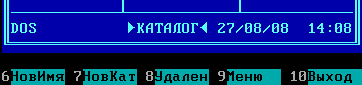
\includegraphics[width=0.5\textwidth]{patterns/01_helloworld/Norton_Commander_v5_51.png}
\caption{Norton Commander 5.51 \emph{localisé}}
\end{figure}
% note to translators: if you know such examples of MS-DOS programs 'localized' to your native language,
% please tell me, maybe I will add more screenshots.

Peut-être que cela s'est produit pour d'autres langages durant cette période.

\myindex{Borland Delphi}
En ce qui concerne Delphi, la taille de la chaîne de caractères doit elle aussi être ajustée.
